\documentclass{article}
\usepackage{tikz}
\usetikzlibrary{arrows.meta,positioning}
\title{Theorema Aureum 143 -- YM Tower Proof Map}
\date{2026-06-15}
\begin{document}\maketitle
\section*{KP Chain}
\begin{tikzpicture}[node distance=2cm,box/.style={draw,rounded corners,minimum width=3cm,minimum height=0.9cm,text centered},arr/.style={-{Stealth},thick}]
  \node[box](D4){$D_4$: $\beta_0\in(2.07,2.08)$};
  \node[box,right=of D4](D5){$D_5$: $w_1\le\tfrac{107}{756}$};
  \node[box,right=of D5](D6){$D_6$: $\tfrac{107}{756}<\tfrac{1}{7}$};
  \node[box,below=1.2cm of D5](KP){KP summable};
  \draw[arr](D4)--(D5); \draw[arr](D5)--(D6);
  \draw[arr](D4)--(KP); \draw[arr](D5)--(KP); \draw[arr](D6)--(KP);
\end{tikzpicture}

Axioms: \texttt{\{propext, Classical.choice, Quot.sound\}}.
Zero \texttt{sorry}.
\end{document}
